\section{Evaluation}
\label{sec:evaluation}
We evaluated our ranking techniques using a large dataset
from real web services in deployment with data from real users.
We trained models on all Zagat-rated establishments in the US,
using the Zagat editorial score as ground truth label.
We performed three sets of experiments:
\squishlist
  \item Evaluation of accuracy and mean squared error of various classifiers
  \item Evaluation of performance of average user review rating
  \item Comparison of performance of SolocoRank-generated scores and various other metrics
\squishend
We also report on the dataset used and the experimental setup.

\subsection{Classifier Performance}
\label{sec:classifierperformance}
We evaluated a variety of classifiers and measured their accuracy and mean squared error.
Out of all of the Zagat-rated restaurants in the United States,
we randomly split half into a training set and half into a testing set.
Each classifier was trained on the training set, and then evaluated on the test set.
Mean squared error is only plotted for testing error.

\begin{figure}
  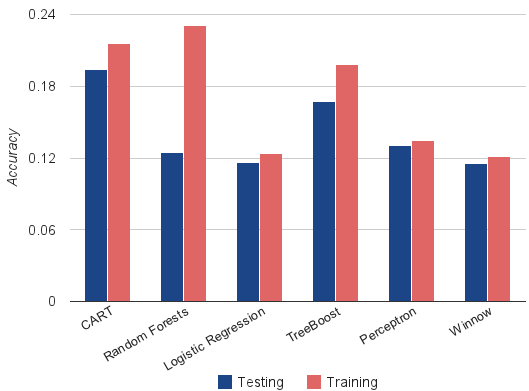
\includegraphics[width=.5\textwidth]{fig/classifieraccuracy.png}
  \caption{Classifier accuracy for various classifiers. 
  CART decision trees have the highest classification accuracy,
  predicting the exact Zagat score 19\% of the time.}
  \label{fig:classifieraccuracy}
\end{figure}

Figure \ref{fig:classifieraccuracy} shows the classifer accuracy.
Note that Zagat scores are discrete values from 0 to 30.
Thus, this chart represents each classifier's ability to
predict the Zagat score exactly.
Classification and regression trees (CART) are able to accurately 
predict the exact Zagat score about 19\% of the time.
CART was able to predict the Zagat score within $\pm1$ point, 44\% of the time.

\begin{figure}
  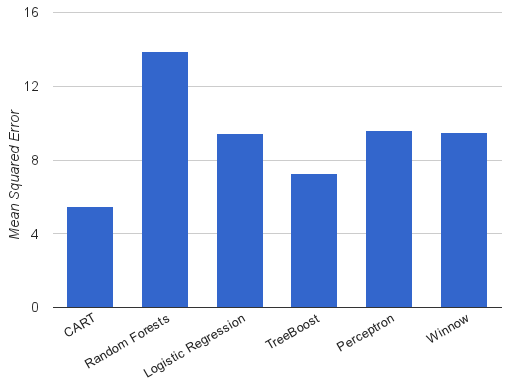
\includegraphics[width=.5\textwidth]{fig/meansqerror.png}
  \caption{Mean squared error of various classifiers on test set.
  CART decision trees have the lowest mean squared error of 5.46.}
  \label{fig:classifiermeansqerror}
\end{figure}

Figure \ref{fig:classifiermeansqerror} shows the mean squared error from each classifier.
CART again does the best along this metric.
With a mean square error of 5.46, this means that CART predictions are on average only a
few points off of the true Zagat score.

In general, decision tree-based classifiers performed better than others.
Trees are able to capture complex relationships, as well as produce a human-readable
tree that describes such relationships.
For example, a tree can capture the trend that checkin-based services 
are much more commonly used in certain cities than other places.
However in order to train our CART model, it took on the order of days to weeks depending
on the parameters.
The rest of the paper will evaluate \emph{SolocoRank} using the TreeBoost model with limited
complexity, allowing us to perform more evaluations with shorter training time.
As shown in Figures \ref{fig:classifieraccuracy} and \ref{fig:classifiermeansqerror},
TreeBoost performs close to the performance of CART.
In all experiments, we limited TreeBoost to 50 rounds of boosting,
where each tree was limited to a depth of 6.

\subsection{Generating Test Sets of Restaurants}
\subsubsection{Data Collection}
Our evaluation data consists of 150 test sets of five restaurants each.
In order to generate these sets, we divided all restaurants in New York City into comparable categories.

Once we had comprehensive restaurant coverage in each comparable category,
each comparable category was further divided into sets of five, labeled by the original category.
If a comparable category contains less than five elements, that category was disgarded.
We then selected 150 sets at random from all sets to compose the evaluation data set.
Thus, our evaluation data set distribution is approximately close to the distribution of restaurants
in existence in the city of New York.
However, note that this distribution of restaurants is likely different 
from the distribution of search queries on a mapping site.

This process was performed in order to produce query-independent sets of 
restaurants in the same comparable category.
Each set contains five random restaurants without any bias from an existing search engine.

\begin{figure}
  \begin{center}
    \begin{tabular}{|c|c|}
      \hline
      Restaurant Name           & Rating \\
      \hline
      \hline
      Shanghai Gourmet          & 3 \\
      \hline
      Xi'an Famous Foods        & 4 \\
      \hline
      Fong Inn Too              & 3 \\
      \hline
      Shu Jiao Fu Zhou Cuisine  & 3 \\
      \hline
      Oriental Kitchen          & 1 \\
      \hline
    \end{tabular}
  \end{center}
  \caption{Example of a test set in a comparable category: 
  cheap Chinese restaurants in New York City}
  \label{fig:testset}
\end{figure}

\subsubsection{Obtaining Relevance Ratings}
Each of these sets were then scored by three unique raters.
The rater was asked to assign a "relevance score" on a scale from [1-5] 
to each of the restaurants in a test set according to the following guidelines:
\squishlist
	\item 5 - You would frequently go or recommend this place to others
	\item 4 - You would definitely try this place at least once
	\item 3 - You may go to this place if it is in your area
	\item 2 - You would go to this place only in dire circumstances
	\item 1 - You would never go to this place
  
\squishend
Raters were encouraged to research these restaurants using a variety of online resources, 
including restaurant recommendations, Web search, newspaper articles, and user reviews.
The score may include a number of considerations, 
including the quality of food, cleanliness, service, and popularity. 
In the case where the restaurant type was misclassified 
(i.e. a French restaurant in a set of Chinese restaurants), 
the rater could still score the rest of the set, while ommiting the score of the misclassified restaurant.

Note that the rater was not asked to strictly order the restaurants. 
The set of five restaurants provides a frame of reference, but scores did not have to be unique.
Thus it was common to see repeat scores within a single set.
For example, a list of five restaurants may yield the scores [3, 4, 3, 3, 1]
as shown in Figure \ref{fig:testset}.

After each test set was scored by three raters, we ultimately took the majority 
as the final relevance score.
For example, if the raters returned: [3,4,3,3,1], [3,4,3,2,2], and [2,4,3,4,1], 
the final score was [3,4,3,x,1].
The fourth restaurant was disgarded from the set, 
because the raters could not come to a majority agreement.
We found that disagreement was generally very rare.

\subsubsection{Calculating Ranking Quality}
We evaluate a particular ranking method, such as \emph{SolocoRank}, by using the standard NDCG metric.
Given the relevance list of restaurants $R$ of a predicted ranking, 
the Discounted Cumulative Gain (DCG)
at position $p$ is given by $DCG_p(R) = \sum_{i=1}^{p}(2^{R_i}-1)/log_2(i+1)$.
This particular formulation of the DCG takes into account the rankings of the $p$ positions
and gives results at the top of the list more weight.
The normalized DCG (NDCG) can then be defined as $NDCG_p(R) = DCG_p(R)/DCG_p(I)$, where $I$ is
the relevance labeling of the ideal ranking.
Because each test set contains 5 restaurants, we always calculate NDCG for $p=5$.

\subsection{Raw User Review Scores}
In this section, we characterize raw user-generated reviews and 
evaluate the ability for user reviews to properly order restaurants.
User reviews are normalized on a scale from [0-100] and we simply take the average
review score across all reviews.
This average rating was then used to order our evaluation test sets,
without the use of machine learning.

\begin{figure}
  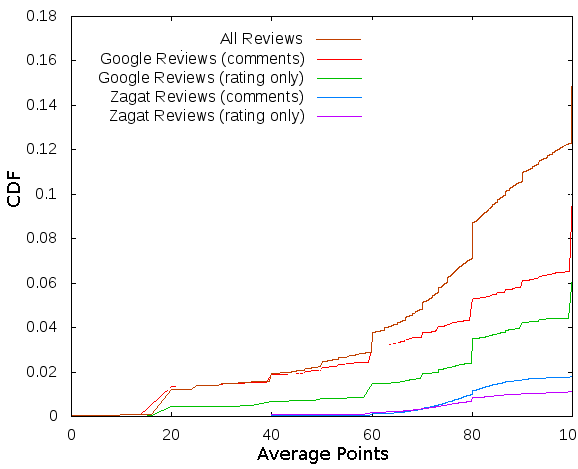
\includegraphics[width=0.5\textwidth]{fig/graph-avgpoints2.png}
  \caption{Cumulative distribution function (CDF) of average review scores in our database.
  CDF is shown separately for reviews with comments and reviews with only a star rating.
  CDF is also shown separately for Google Maps reviews and reviews from Zagat.com.
  Reviews are a sparse data set and users tend to have high score biases.}
  \label{fig:reviewscoredistribution}
\end{figure}

Figure \ref{fig:reviewscoredistribution} shows the cumulative 
distribution function of average review scores of establishments in the US.
The graph clearly shows that users tend to have strong biases towards high scores.
This property lowers the amount of information gained from users, while inflating scores shown to users.
Second, reviews are a scarce data source.
Roughly 12\% of establishments in New York City have any review scores associated with it.
Note that this is a percentage of all registered establishments in the city,
and not just bars and restaurants.

We then calculated the NDCG of our evaluation set,
using average user review score as the ranking metric.
Section \ref{sec:evaluation} describes our experimentation setup in greater detail.
As expected, ordering by average user review score provides
higher quality ordering of restaurants when compared to random ordering,
as shown in Figure \ref{fig:ndcgtable}.
The experiment yielded an average NDCG value of 0.8831,
across our evaluation data set, described in Section \ref{sec:setup}.

There were a few limitations to the approach.
In our experiments, an establishment with no score is treated 
the same as an establishment with a score of 0.
However, this may not reflect reality, as it inherently 
discriminates against new restaurants.
In the case where we had no reviews, there was no way to leverage other
forms of data to relatively order the restaurant.

Furthermore, the signal proved to be unreliable in the case where
there were only a few reviews. 
Suppose we were trying to relatively order two places, 
each with only a handful of reviews.
The average user review score is then a very noisy signal,
and it is very unlikely that both places were reviewed by the same people.

One could incorporate review counts in a more complex heuristic
for ranking.
However, this approach raises additional problems.
One could encounter a self-referring loop, where restaurants with many reviews
are reinforced at the top of search results and become hard to dislodge.
It also introduces the question of what heuristic should be used to 
combine this information in a way that reflects what users want.
\emph{SolocoRank} aims to solve exactly this problem by applying machine learning
to the problem.
In the next Section, we introduce the methodology behind \emph{SolocoRank},
which addresses these limitations and leads to further improvements in NDCG.

\subsection{NDCG Summary}
\begin{figure}
  \begin{center}
  \begin{tabular}{|c|c|}
    \hline
    Ranker            & NDCG  \\ \hline \hline
    Random            & 0.8393\\ \hline
    User Reviews      & 0.8831\\ \hline
    PlaceRank         & 0.8947\\ \hline
    \emph{SolocoRank}        & 0.8891\\ \hline
    \emph{SolocoRank}*PlaceRank  & 0.9011\\ \hline
  \end{tabular}
  \end{center}
  \caption{Average NDCG values across all test sets in our evaluation data.
  Due to high relevance score bias from our raters, NDCG values are biased high.
  However, both \emph{SolocoRank} and Google's current PlaceRank algorithms outperform
  using user-review scores. A linear combination of \emph{SolocoRank} and PlaceRank
  produces the highest quality scores.}
  \label{fig:ndcgtable}
\end{figure}

Figure \ref{fig:ndcgtable} summarizes average NDCG scores across our evaluation test sets.
Random ordering produces a rather high NDCG value of 0.839, 
due to the high score bias from our raters. 
Many times raters would return sets where a number of restaurants have either
high scores or identical scores. 
Due to the way NDCG is calculated, restaurants with the same relevance
can be ordered arbitrarily and still be perfectly ordered.
Because of this bias, the raw NDCG value provides little insight into
performance gains of \emph{SolocoRank}. In later sections, we use
non-parametric evaluations to highlight performance gains.
Even with such a high NDCG bias, we see that both \emph{SolocoRank} and
Google's current algorithm, PlaceRank, outperform user reviews.
As a point of comparison when we perform a linear combination of \emph{SolocoRank} and PlaceRank,
we show consistently better performance compared to any other individual signal.

\subsection{SolocoRank Quality}
In this section, we use the TreeBoost classifier to evaluate the NDCG
of \emph{SolocoRank} on the evaluation data.
We compare the performance of \emph{SolocoRank} to random ordering, average user review score,
and PlaceRank, Google's current state of the art algorithm.
Although our evaluation set contains only restaurants and bars in New York City,
our \emph{SolocoRank} model is trained on all Zagat-rated places in the United States.

\begin{figure}[h]
  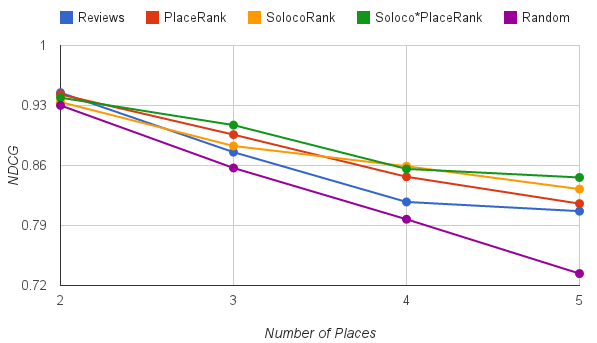
\includegraphics[width=.5\textwidth]{fig/ndcg-vs-numdocs.png}
  \caption{NDCG across varying numbers of documents. 
  \emph{SolocoRank} consistently outperforms using average user review scores.
  Due to the distribution of relevance scores, NDCG values had a high bias.}
  \label{fig:ndcg-vs-numdocs}
\end{figure}

Figure \ref{fig:ndcg-vs-numdocs} graphs the NDCG of the various methods
across different numbers of documents.
In other words, we vary $p \in [2,5]$, where $DCG_p(R) = \sum_{i=1}^{p}(2^{R_i}-1)/log_2(i+1)$.
Note that if all of the documents in the first $p$ elements of $R$
contain the same relevance score from the raters,
then the NDCG will always be 1, regardless of the ranker used.

Thus for lower values of $p$, NDCG values tended to be much higher and closer.
For larger values of $p$, we notice that \emph{SolocoRank} consistently performs better
than user reviews.

\begin{figure}[h]
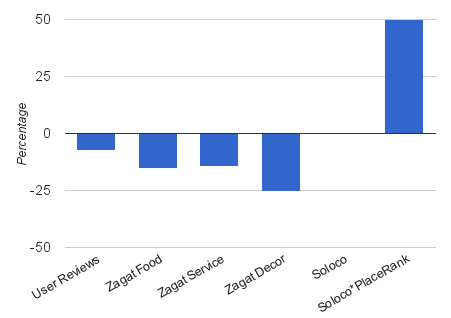
\includegraphics[width=.5\textwidth]{fig/versusplacerank.png}
\caption{When counting the number of test sets for which SolocoRank
had a higher NDCG, we show that each individual review signal performed
worse than SolocoRank by 10-25\%}
\label{fig:versusplacerank}
\end{figure}

Due to the distribution of relevance scores that were assigned in our
evaluation test set, NDCG values had a substantial high bias, even for random ordering.
Thus, it was helpful to perform non-parametric evaluations of each method.
In these evaluations, we counted the number of test sets, where the NDCG is higher
for \emph{SolocoRank}, when compared to the NDCG from average user reviews.
Figure \ref{fig:versusplacerank} shows the percentage improvement in the 
number of test sets with a higher NDCG value when compared to SolocoRank.
For example when SolocoRank was compared to PlaceRank, there were equal
numbers of test sets where the NDCG value was higher for SolocoRank, as
there were test sets where the NDCG value was higher for PlaceRank.
However, it is interesting to note that any individual review signal performed
worse than SolocoRank.
When using user review scores, there was about 10\% fewer test sets with better
NDCG.
Again as a point of comparison, we were able to show 50\% improvement
when SolocoRank was combined with PlaceRank.

\subsection{Information Gain from Social Media}
\begin{figure}[h]
  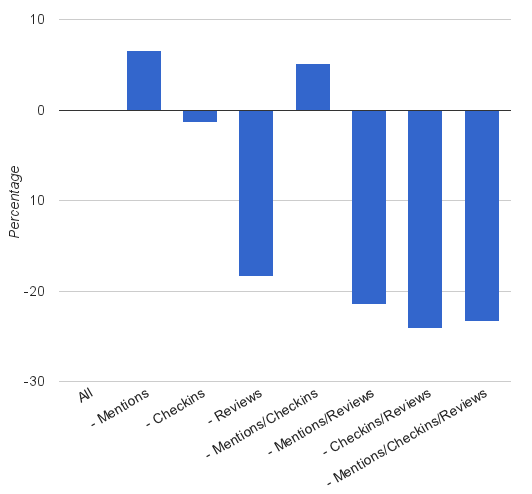
\includegraphics[width=.5\textwidth]{fig/signalselection-accuracy.png}
  \caption{Classifier accuracy without particular features. As expected,
  reviews provide the most information gain. Surprisingly, classifier
  accuracy performs better without \emph{mention} data.}
  \label{fig:signalselection-accuracy}
\end{figure}

We wanted to evaluate the effect of each particular category of signals in 
the final NDCG value.
Figure \ref{fig:signalselection-accuracy} shows the percent change in NDCG, 
compared to the original baseline of using all signals.
As expected, removing reviews severely impaired SolocoRank's NDCG performance.
However, it was surprising to see that the removal of mentions actually improved
NDCG performance.
This negative effect may be caused by the way this signal was produced and encoded.
At the moment, we simply count the number of mentions on Google Plus
and Twitter webpages with a minimum PageRank value.
In the future, we could perform more intelligent sentiment analysis in conjunction with
mentions in order to determine if the mention was negative or positive.
